\documentclass{scrreprt}
\usepackage[margin=0.7in]{geometry} %réduire marges

\usepackage[french]{babel} %en Français
\usepackage[utf8]{inputenc}
\usepackage[colorlinks=true,urlcolor=blue,linkcolor=blue]{hyperref}
\usepackage[T1]{fontenc}
\usepackage[babel=true]{csquotes}
\usepackage{array}
\usepackage{multicol}
\usepackage{hyperref}

\usepackage[pdftex]{graphicx}
\usepackage{epsfig}

\hyphenation{uti-li-sateur}
\begin{document}
\pagenumbering{arabic}

\title{iBalezator}
\subtitle{\textit{Spécifications Techniques de Réalisation}\vspace{-5ex}}
\date{2 avril 2015}
\author{Adrien FERREIRA, Alexandra HOSPITAL}
\maketitle
\tableofcontents \newpage


\chapter{Le projet}
\noindent \textbf{Maitrise d’ouvrage :} Thomas Baspeyras, Fabrice Kordon \newline
\noindent \textbf{Maitrise d’oeuvre :} Adrien FERREIRA, Alexandra HOSPITAL\newline

\section{Contexte}

iBalezator est une application pour terminaux sous iOS 8 qui consiste en un jeu de devinette pour mémoriser la disposition des notes sur le manche d’une guitare. L'application comporte deux modes de jeux :
\begin{itemize}
\item Le mode manche/clavier, dans lequel l'utilisateur lit une question sur le manche et répond sur un clavier
\item Le mode portée/manche, dans lequel l'utilisateur lit une question sur la portée et répond sur le manche.
\end{itemize}

\medbreak

Ce document traite des spécifications techniques de réalisation du projet iBalezator. Il complète le cahier des charges dans lequel les besoins sont spécifiés en détails.\newline

\section{Environnement de développement}
\subsection{Matériel}

Le matériel utilisé est un Mac mini sous MacOS 10.9.5. 
Le développement sera effectué sur la plate-forme de développement Xcode 6.1 en langage Swift, avec possibilité d'inclure des portions de code en Objective-C ou C.

Les tests seront effectués sur un iPod touch MD720NF/A sous iOS 8.1.3. Le déploiement sera fait du Mac vers l'iPod via le logiciel Xcode.

\subsection{Bibliothèques}

Nous utilisons les différentes bibliothèques incluses par défaut pour le Swift. \\
La bibliothèque de son utilisée est audiokit (\url{http://audiokit.io/features/}).


\section{Pré-requis}
\subsection{Jeu sur la guitare}

\bigbreak
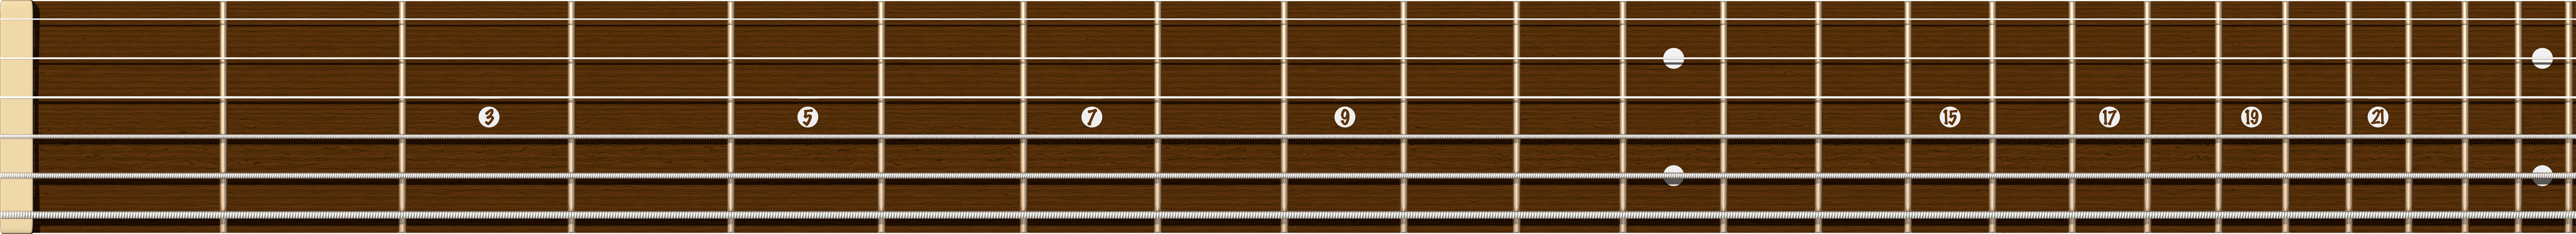
\includegraphics[width=\textwidth]{str-images/neck.png}
\bigbreak

Pour comprendre la description des fonctionnalités de l'application, il est important de comprendre le jeu sur un manche de guitare. \\
Un manche de guitare est composée de 6 cordes (représentées horizontalement sur l'image ci-dessus) et de 24 frettes (verticalement sur l'image).
Les cordes sont, de haut en bas : mi (aigu), si, sol, ré, la, mi (grave). Ce sont les notes jouées pour les cordes dites \enquote{à vide}, c'est-à-dire sans pincer aucune corde sur les cases du manche.\\

 Les notes d'une gamme sont do, do\#, ré, ré\#, mi, fa, fa\#, sol, sol\#, la, la\#, si. Elles sont séparées par un intervalle appelé \enquote{demi-ton}. Par exemple entre do et do\#, nous avons un demi-ton.
Les frettes sont placées tous les demi-tons sur le manche de la guitare. De cette façon entre deux frettes, nous avons toujours un demi-ton. Par exemple pour la corde de mi, la première frette nous donne un fa, la deuxième un fa\#, la troisième un sol, et ainsi de suite.

Pour lire une note sur le manche de la guitare, on doit donc se placer sur la corde en question, puis l'augmenter de demi-ton en demi-ton jusqu'à arriver à la note voulue, à la frette désirée. Par exemple, pour la corde de mi aigu, sur la troisième frette, on obtient un sol (mi augmenté de trois demi-tons dans la gamme).

\subsection{Lecture de notes sur la portée}


\bigbreak
\includegraphics[width=\textwidth]{str-images/note_portee.jpg}
\bigbreak

Une portée est constituée de 5 lignes. 
Les notes peuvent être disposées sur une ligne ou entre deux lignes. Les notes sur la partie basse de la portée sont graves, et celles de la partie haute sont aigues. 
Lorsque les notes sont plus graves ou plus aigues que celles placées dans la portée, on trace des lignes supplémentaires. Sur l'image ci-dessus, des lignes ont été ajoutées du mi au do graves et du la au mi aigus.\\
En mode portée/manche, les notes possibles affichées sur la portée seront celles ci-dessus.
La portée contient 3 otaves. 
Par exemple, du premier mi au deuxième mi, nous avons une octave, c'est-à-dire toutes les notes différentes jusqu'à ce qu'on retombe sur la note de départ.
Le premier mi sera donc appelé mi1, le deuxième mi2, et ainsi de suite.\\
Les notes représentées correspondent aux notes sur le manche de la guitare jusqu'à la 12ème frette. 
Au delà de la 12ème frette, et donc au delà du mi4, les notes sont représentées à l'octave du dessous avec une indication \enquote{8va}.
Par exemple, pour représenter le fa4, nous aurons un fa au même niveau que le fa3, avec l'étiquette \enquote{8va} qui indique que ce fa doit être joué une octave au dessus de celui écrit sur la portée.

\chapter{Implémentation}
\section{Architecture de l'application}
\begin{figure}[h!]
	\includegraphics[width=\textwidth]{str-images/Diagrammedeclasses.png}
	\caption{Diagramme de classes}
\end{figure}

\newpage



\section{Architecture}
La strucure globale de notre application répond au patron de conception MVC.
Chaque écran fait intervenir plusieurs vues : manche (NeckView), barre de score (ScoreView), clavier de réponse (KeyboardView), portée (StaffView).
L'application est composée de deux écrans correspondant aux deux modes de jeu de l'application.
Les deux modes sont :
\begin{itemize}
	\item Clavier : qui contient les vues ScoreView, NeckView et KeyboardView.
	\item Portée : qui contient les vues ScoreView, StaffView et NeckView.
\end{itemize}
Ces deux modes partagent la même instance des classes NeckView et ScoreView.

La classe Note est utile pour stocker le couple <frette, corde>, elle donne également plusieurs méthodes qui permettent de convertir une note en d'autres informations utiles. 
Il est important de créer un clivage entre la NeckView qui opère sur des coordonnés et le reste de l'application qui lui doit manipuler des Notes. 
Le NeckController est la classe qui permet la conversion des coordonnés en instance de la classe Note.

À chaque instance d'une vue correspond une instance d'un controleur homonyme qui lui est associé.
Les controleurs de vue sont tous liés à un controleur principal nommé GameController.
La logique est de toujours déléguer les traitements spécifique à une vue au contrôleur homonyme qui lui est associé.
On peut cependant s'autoriser des appels de méthode entre le GameController et les vues.

Le SoundController est à voir comme un sevice offrant la possibilité de jouer des notes.
Il doit permettre l'abstraction de la bibliothèque audio utilisée.
Il doit pouvoir, comme tous les autres contrôleur, opérer avec des inctances de la classe Note.

Le Modèle de l'application est composé de deux instances différentes : une pour chaque mode de jeu.
La raison pour laquelle il faut avoir recours à l'héritage est qu'une portée présente un ensemble de notes contrairement au manche qui lui n'en représente qu'une à la fois.
Voilà pourquoi la classe GameStaffModel possède un tableau de Note alors que le GameKeyboardModel lui n'en stocke qu'une. 
Les attributs restant étant communs aux deux modes de jeu, ils sont obtenus par héritage.


\section{Fonctionnalités}

\subsection{GameController}

Cette classe est responsable de la logique du jeu. C'est elle qui vérifie les réponses données par \mbox{l'utilisateur}, mettre à jour son score, déléguer l'actualisation des vues au contrôleurs adéquats.
Ce contrôleur contient également un attribut qui précise le mode courant du jeu : clavier/manche ou portée/manche dans curMode. 
\begin{itemize}
\item changeMode : cette méthode réagence l’écran avec les vues nécessaires. La variable curMode est mise à jour.
\item showHelp : cette méthode vide l’écran pour n’afficher que l’écran d’aide (certainement une WebView).


\item CheckAnswerKeyboard prend en paramètre la note sélectionnée par l’utilisateur sur le clavier. Il fait correspondre la note actuellement présentée sur le manche en interrogeant le modèle (getCurNote).
\item CheckAnswerNeck prend en paramètre la note sélectionnée par l’utilisateur sur le manche. Il fait correspondre la note actuellement présentée sur la portée en interrogeant le modèle.

En fonction du résultat de la fonction Check, le GameController met à jour le score de l’utilisateur dans le GameModel. Si la réponse est mauvaise le GameControler stocke également la note erronée dans le GameModel (wrongAnswer). 
 
\end{itemize}

\subsection{GameModel}

Les données seront stockées dans ce modèle, lui-même divisé en deux classes (par héritage) :
\begin{itemize}
\item GameKeyboardModel : contient pour seul attribut la note courante à deviner.
\item GameStaffModel : contient un ensemble de notes présentées sur la portée, et l'indice dans cet ensemble de la note courante à deviner.
\end{itemize}

\subsection{KeyboardController}

Cette classe a pour vocation de réceptionner les événements en provenance de KeyboardView et de lancer les fonctions d’actualisation sur cette même vue.\\
handlerTap reçoit en paramètre le nom de la note tapée au clavier et délègue la vérification de la question posée au GameController. Ce handler peut éventuellement être déplacé dans le GameController pour des raisons de praticité.


\subsection{KeyboardView}
C’est cette vue qui représente le clavier sur lequel l’utilisateur saisit sa réponse en mode Manche/Clavier.\\
Cette vue doit intercepter le tap de l’utilisateur effectué sur un clavier (UIButton
ou SegmentedConrol). Les événements en provenance de cette vue sont dirigés vers l’objet KeyboardController.
A priori aucun traitement à destination de cette vue n’est attendu.\\
Cette vue doit représenter 35\% de la taille de l’écran.


\subsection{NeckController}

Cette classe a pour vocation de réceptionner les événements en provenance de NeckView et de lancer les fonctions d’actualisation sur cette même vue. Elle contient des méthodes de conversion :
\begin{itemize}
\item coordToPosition : lorsque l'utilisateur tape sur le manche, les coordonnées correspondant à son tap sont données à une fonction qui a pour but de la transformer en position sur le manche. La position sur le manche est un couple <frette, corde>.
\item Cette fonction traduit une position (couple <frette, corde>) sur le manche en note. Chaque frette représentant un demi-ton, on augmente la note de la corde donnée d’autant de demi-tons que le numéro de la frette, modulo les douze notes différentes. 
\item noteToCoord : Une note, selon le couple <frette, corde> est traduite en coordonnées sur le manche
\item findNote : Cette méthode trouve une note définie par le couple <frette, corde> grâce à une chaîne de caractères passée en paramètres en fonction de la partie visible du manche. 
De cette façon, lorsqu'une mauvaise réponse est données par l'utilisateur sur le clavier en mode manche/clavier, cette fonction trouve une note correspondant à cette mauvaise réponse pour afficher le marqueur rouge.  
\item getClosestFret : lors du défilement du manche par l'utilisateur, il est possible que le bord gauche de l'écran ne soit pas aligné sur une frette. À la fin de l'animation du déplacement, on veut caler le bord gauche de l'écran sur une frette du manche. Cette méthode est utilie pour touver la frette la plus proche du bord gauche de l'écran. Si l'on considère que le bord gauche de l'écran est entre deux frettes, il faudra alors qu'il trouve la plus proche. Soit celle à gauche du bord gauche de l'écran (frette encore invisible donc) soit celle à droite.
\end{itemize}

\subsection{NeckView}

Cette classe est une UIScrollView pour permettre à l’utilisateur de faire défiler le manche. 
Cette UIScrollView contiendra elle-même une UIImage qui affiche effectivement l’image du manche.
Les événements en provenance de cette vue seront dirigés vers l’objet NeckController.
Cette vue permet d’afficher des pastilles de couleur sur les différentes notes du manche grâce à des méthodes d'ajout et de suppression : addMarker, deleteMarker. Ces méthodes ne doivent manipuler que des coordonnées du tap de l'utilisateur sur la vue.\\
Cette classe contient des méthodes d'ajout, de suppression et de mise à jour d'une pastille sur le manche. \\
Cette vue représente 55\% de la taille de l'ecran.

\subsection{Note}

Pour pouvoir positionner une note de manière unique sur le manche, il faut avoir le couple <corde, frette>. On ne peut se contenter d'un nom de note, car cette note est disponible à plusieurs endroits sur le manche. Le but de cette classe est donc de mémoriser et convertir ce couple en une autre information utile (i.e : nom de note simple, note en valeur absolue, …).\\
positionToNote : cette méthode convertit le couple <corde, frette> en un nom de note (ex : do, sol, ré\#).

\subsection{ScoreController}

Cette classe a pour vocation de lancer les fonctions d’actualisation sur ViewController.
changeNotesStaff : cette fonction interroge le GameModel pour connaître les notes à afficher sur la portée. Il peut ainsi invoquer les méthodes : highlightNextNote, showWrongAnswer, showGoodAnswer et addNewNote. 


\subsection{ScoreView}

Cette vue présente la barre de progression de l’utilisateur. Elle affiche également un bouton (UIButton) pour que l’utilisateur puisse changer de mode.\\
Les événements en provenance de cette vue sont dirigés vers l’objet ScoreController.
Cette vue doit permettre de mettre à jour le pourcentage de bonnes/mauvaises réponses dans la barre de progression. Cette vue a une hauteur fixe de 50 points imposés par Apple.


\subsection{SoundController}

Cette classe est l’interface pour le jeu de son. Elle doit abstraire et simplifier l’utilisation d’une bibliothèque de lecture de son.\\
playNote : cette fonction prend une note en paramètre, convertit cette note en fréquence grâce à la méthode noteToFrequence et lance la lecture d’un son grâce à cette fréquence trouvée.

\subsection{StaffController}

Cette classe a pour vocation de lancer les fonctions d’actualisation sur ViewController.\\
changeNotesStaff : cette fonction interroge le GameStaffModel pour connaître les notes à afficher sur la portée. Il peut ainsi invoquer les méthodes : 
\begin{itemize}
\item highlightNextNote : surbrillance jaune
\item showWrongAnswer : surbrillance rouge
\item showGoodAnswer : surbrillance verte
\item putNoteOnStaff : Cette méthode doit prendre un object Note en paramètre et la placer la note correctement sur la portée. 
Elle doit aussi gérer l'affichage de lignes supplémentaires basses et hautes sur la portée si la Note en paramètre le nécéssite. 
Lorsqu'une note est très aigue (i.e : Fa4), on doit aussi faire apparaître sur la portée une indication de lire la note à l'octave supérieure par rapport à ce qui est affiché sur la portée. Ceci grâce au signe \enquote{8va}.
\end{itemize}

Le StaffController est lui même relié au GameController qui va invoquer les méthodes nécessaires en fonction de l’évolution du jeu.

\subsection{StaffView}

Cette vue est une UIImageView, elle affiche l’image de la portée. Les notes sont affichées par superposition sur cette image de base. Les événements en provenance de cette vue sont dirigés vers l’objet StaffController.
Cette vue doit permettre d’afficher des notes données en paramètre sur la portée et de colorer ces notes en rouge, vert, ou jaune. Cette vue est censée ne retourner/recevoir que des coordonnées, jamais des objets Note.

\subsection{Changement de mode}



\end{document}
